\documentclass{beamer}

% ====================
% Packages
% ====================

\usepackage[size=custom, width=160,height=90, scale=1.6]{beamerposter}

\usepackage[T1]{fontenc}
\usepackage[utf8]{luainputenc}
\usepackage{lmodern}
\usepackage[sfdefault]{roboto}


\usetheme{gemini}
\usecolortheme{mit}

\usepackage{graphicx}
\usepackage{booktabs}
\usepackage{tikz}
\usepackage{pgfplots}
\pgfplotsset{compat=1.14}

\usepackage{anyfontsize}
\usepackage{fontawesome5}

\usepackage{lipsum}
\usepackage[square]{natbib}
\usepackage{tabularx}
\usepackage{siunitx}
\sisetup{detect-all}
\usepackage{amsfonts}
\usepackage{amsmath}
\usepackage{amssymb}

\hyphenpenalty=10000

% ====================
% Lengths
% ====================

% If you have N columns, choose \sepwidth and \colwidth such that
% (N+1)*\sepwidth + N*\colwidth = \paperwidth

\newlength{\sepwidth}
\newlength{\colwidth}

% 2 columns
%\setlength{\sepwidth}{0.025\paperwidth}
%\setlength{\colwidth}{0.4625\paperwidth}
\setlength{\sepwidth}{0.025\paperwidth}
\setlength{\colwidth}{0.3\paperwidth}

\newcommand{\separatorcolumn}{\begin{column}{\sepwidth}\end{column}}

% ====================
% Title
% ====================

\title{Monitoramento de incêndio em Goiás com apoio da ciência cidadã}

\author{Izadora Bernardi e Pedro Lucas Siqueira da Paixão}

\institute[shortinst]{Bacharelado em ciência da computação, IF Goiano - Campus Rio Verde}

% ====================
% Footer (optional)
% ====================

\footercontent{
    \href{https://github.com/IzaBern/mapa-monitoramento-incendio}{\faGithub\hspace{0.5ex} IzaBern/mapa-monitoramento-incendio}
    \hspace{5cm}
    \href{mailto:izadora.bernardi@estudante.ifgoiano.edu.br}{\faEnvelope\hspace{0.5ex} izadora.bernardi@estudante.ifgoiano.edu.br}
    \hspace{5cm}
    \href{mailto:srpedrogames20@gmail.com}{\faEnvelope\hspace{0.5ex} srpedrogames20@gmail.com}
}
% (can be left out to remove footer)

% ====================
% Logo (optional)
% ====================

% use this to include logos on the left and/or right side of the header:
% Left: institution
\logoright{
\includegraphics[height=7cm]{logos/logo_if.png}}
% Right: funding agencies and other affilations 
%\logoright{\includegraphics[height=7cm]{logos/NSF.eps}}
% ====================
% Body
% ====================

\begin{document}
%\large

	\begin{frame}[t]
		\begin{columns}[t]
			
			%%%%%%%%%%%%% Primeira coluna
			\separatorcolumn			
			\begin{column}{\colwidth}
				% %%%%%%%%%%%%% Resumo
			    % \begin{block}{Resumo}    
			    % 	\small{\lipsum[1]}
			    % \end{block}
			
				%%%%%%%%%%%%% Introdução
			    \begin{block}{Introdução}
			            Tendo em vista as previsões de impactos do El niño para o período de novembro de 2026 a fevereiro de 2027, tais como calor extremo para o norte e enchentes para o sul do país, torna-se relevante a pesquisa e o desenvolvimento de soluções tecnológicas que visam a redução dos principais efeitos colaterais do evento climático.

						As previsões para região centro-oeste giram em torno de altas temperaturas e períodos de seca prolongada, fatores que somados resultam em um risco maior de incêndios. Pensando nisso, esse artigo propõe um software de mapeamento de focos de incêndio no estado de Goiás, com a participação da população no registro das ocorrências.
			        
			    \end{block}
			
				%%%%%%%%%%%%% Trabalhos relacionados
			    \begin{block}{Trabalhos relacionados}
					O artigo ~\cite{teguh2021android} é o trabalho científico mais relacionado com o projeto, pois inclui o uso de GNSS e GPS para registro da localização geográfica, utilização de metadados EXIF para registro da data e horário da foto capturada pelo cidadão, uma etapa de validação dos dados por um administrador, visualização no mapa usando Google Maps API e notificação dos bombeiros, além de funcionar offline. Nosso artigo deve basear a arquitetura em grande parte nesse trabalho, com algumas diferenças pontuais.

					O ~\cite{maillard2024citizen} se relaciona com o trabalho na parte de ciência cidadã, na qual centenas de voluntários coletaram registros de incêndios, desmatamento, água e biodiversidade. Um ponto muito relevante desse artigo é a etapa de verificação de falsos positivos, algo que deve ser prioridade no nosso trabalho, pois um registro falso positivo pode deslocar os bombeiros para uma região sem necessidade.

					Por fim, a classificação e imagens do projeto MapBiomas~\cite{mapbiomas2024cerrado} serviram de base para a identificação e categorização das principais vegetações da região.

			    \end{block}
			
			\end{column}
			
			%%%%%%%%%%%%% Segunda coluna
			\separatorcolumn
			\begin{column}{\colwidth}
				%%%%%%%%%%%%% Metodologia
				\begin{alertblock}{Metodologia}
					\begin{figure}
			            \centering
			            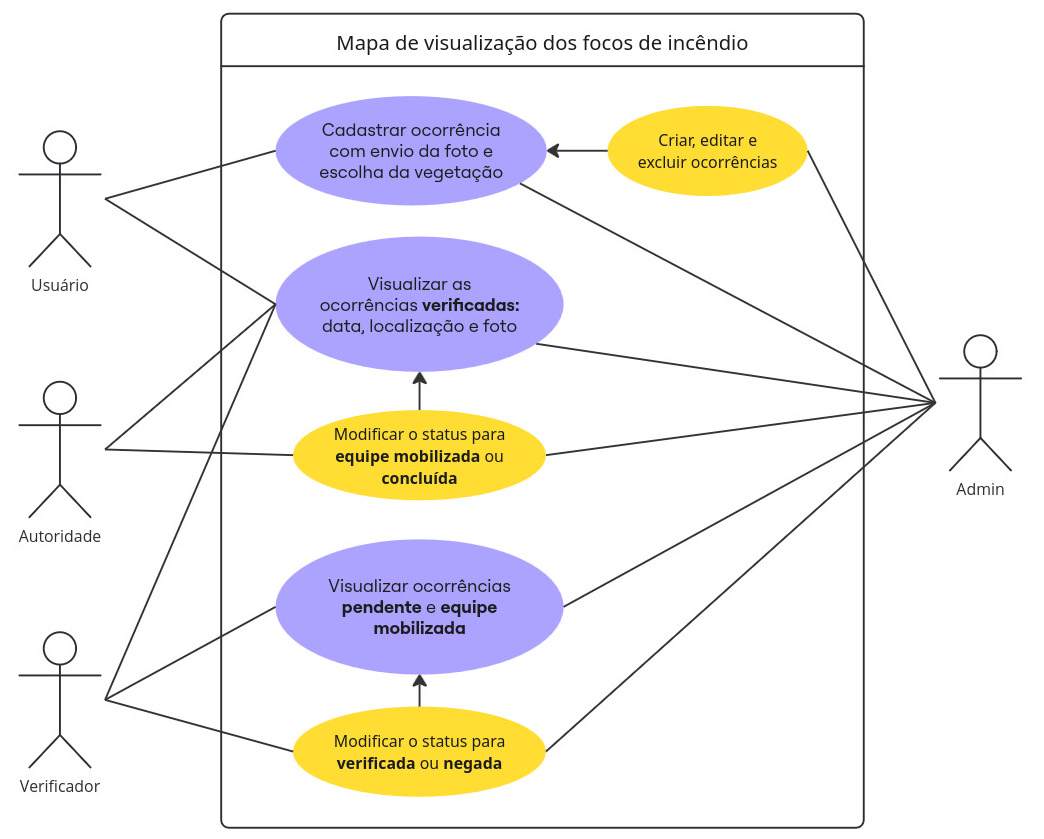
\includegraphics[width=\columnwidth]{figures/casos_de_uso.jpg}
			            \caption{Diagrama de casos de uso.}
			            \label{fig:caso_uso}
			        \end{figure}
					
				\end{alertblock}
			
				% \begin{exampleblock}{A highlighted block containing some math}
					
				% 	A different kind of highlighted block.
					
				% 	$$
				% 	\int_{-\infty}^{\infty} e^{-x^2}\,dx = \sqrt{\pi}
				% 	$$
					
				% 	Interdum et malesuada fames $\{1, 4, 9, \ldots\}$ ac ante ipsum primis in
				% 	faucibus. Cras eleifend dolor eu nulla suscipit suscipit. Sed lobortis non
				% 	felis id vulputate.
					
				% 	\heading{A heading inside a block}
					
				% 	Praesent consectetur mi $x^2 + y^2$ metus, nec vestibulum justo viverra
				% 	nec. Proin eget nulla pretium, egestas magna aliquam, mollis neque.
					
				% 	\heading{Another heading inside a block}
					
				% 	Sed augue erat, scelerisque a purus ultricies, placerat porttitor neque.
				% 	Donec $P(y \mid x)$ fermentum consectetur $\nabla_x P(y \mid x)$ sapien
				% 	sagittis egestas. Duis eget leo euismod nunc viverra imperdiet nec id
				% 	justo.
					
				% \end{exampleblock}
			\end{column}
			
			%%%%%%%%%%%%% Terceira coluna
			\separatorcolumn
			\begin{column}{\colwidth}
			    
			    % %%%%%%%%%%%%% Resultados
			    % \begin{block}{Resultados}
			    %     \begin{figure}
			    %         \centering
			    %         \includegraphics[width=\columnwidth]{figures/ft.jpg}
			    %         \caption{Fourier transform can be applied on cats.}
			    %         \label{fig:ftcat}
			    %     \end{figure}
			    % \end{block}
			
				% %%%%%%%%%%%%% Conclusão
			    % \begin{block}{Conclusão}  
			    % 	Lorem ipsum dolor sit amet, consectetuer adipiscing elit. Ut purus elit, vestibulum ut, placerat ac,
			    % 	adipiscing vitae, felis. Curabitur dictum gravida mauris. Nam arcu libero, nonummy eget, consectetuer
			    % 	id, vulputate a, magna. Donec vehicula augue eu neque.
			    % \end{block}    
			
			    \begin{block}{Referências}    	
				%	    \nocite{*}
					\footnotesize{\bibliographystyle{apalike}\bibliography{references}}
			    \end{block}
			    
			\end{column}
			
			\separatorcolumn
		\end{columns}
	
	\end{frame}
	
\end{document}
